\chapter{Estado del arte}
\label{chap:estadodelarte}

\lettrine{E}{}n el contexto actual del desarrollo de software, la incorporación de herramientas como \textbf{GitHub Copilot} y \textbf{OpenAI Codex} ofrecen la oportunidad de simplificar la creación de código con la asistencia de la inteligencia artificial. Estas herramientas se basan en modelos de lenguaje altamente experimentados, los cuales han sido entrenados con grandes volúmenes de datos de código. Este sistema no solo incrementa la eficacia al reducir las tareas repetitivas, sino que también promueve un enfoque más natural hacia la programación. En este capítulo se abordará el impacto y la implementación de estas modernas técnicas de programación en la industria del software.


\section{GitHub Copilot}

GitHub Copilot \cite{GitHubCopilot} (figura \ref{fig:1_MuestraCopilot}), desarrollado por GitHub tras su adquisición por Microsoft en 2018, representa una innovación significativa en la asistencia a la codificación mediante inteligencia artificial. Implementada a mediados de 2021, esta herramienta se integra en entornos de desarrollo como Visual Studio, Neovim o los \acrshort{IDE}s de JetBrains, dando lugar a sugerencias de código en tiempo real.

El origen de GitHub Copilot se basa en el modelo de lenguaje Codex de OpenAI, una versión especializada del conocido \acrshort{GPT}-3. Este modelo está diseñado para comprender y generar código en una variedad de lenguajes de programación, captando el contexto y la intencionalidad detrás de las entradas de los usuarios para ofrecer sugerencias pertinentes y funcionales.

Desde que se lanzó, más de 1.2 millones de desarrolladores han utilizado Copilot, resaltando su eficiencia en Python, con alrededor del 40 \% de sus sugerencias siendo usadas por los usuarios. Aunque puede crear nuevo código, la herramienta debe mejorar la precisión y relevancia de sus sugerencias para ser útil en entornos donde la exactitud es crucial.

\begin{figure}[htbp!]
  \centering
  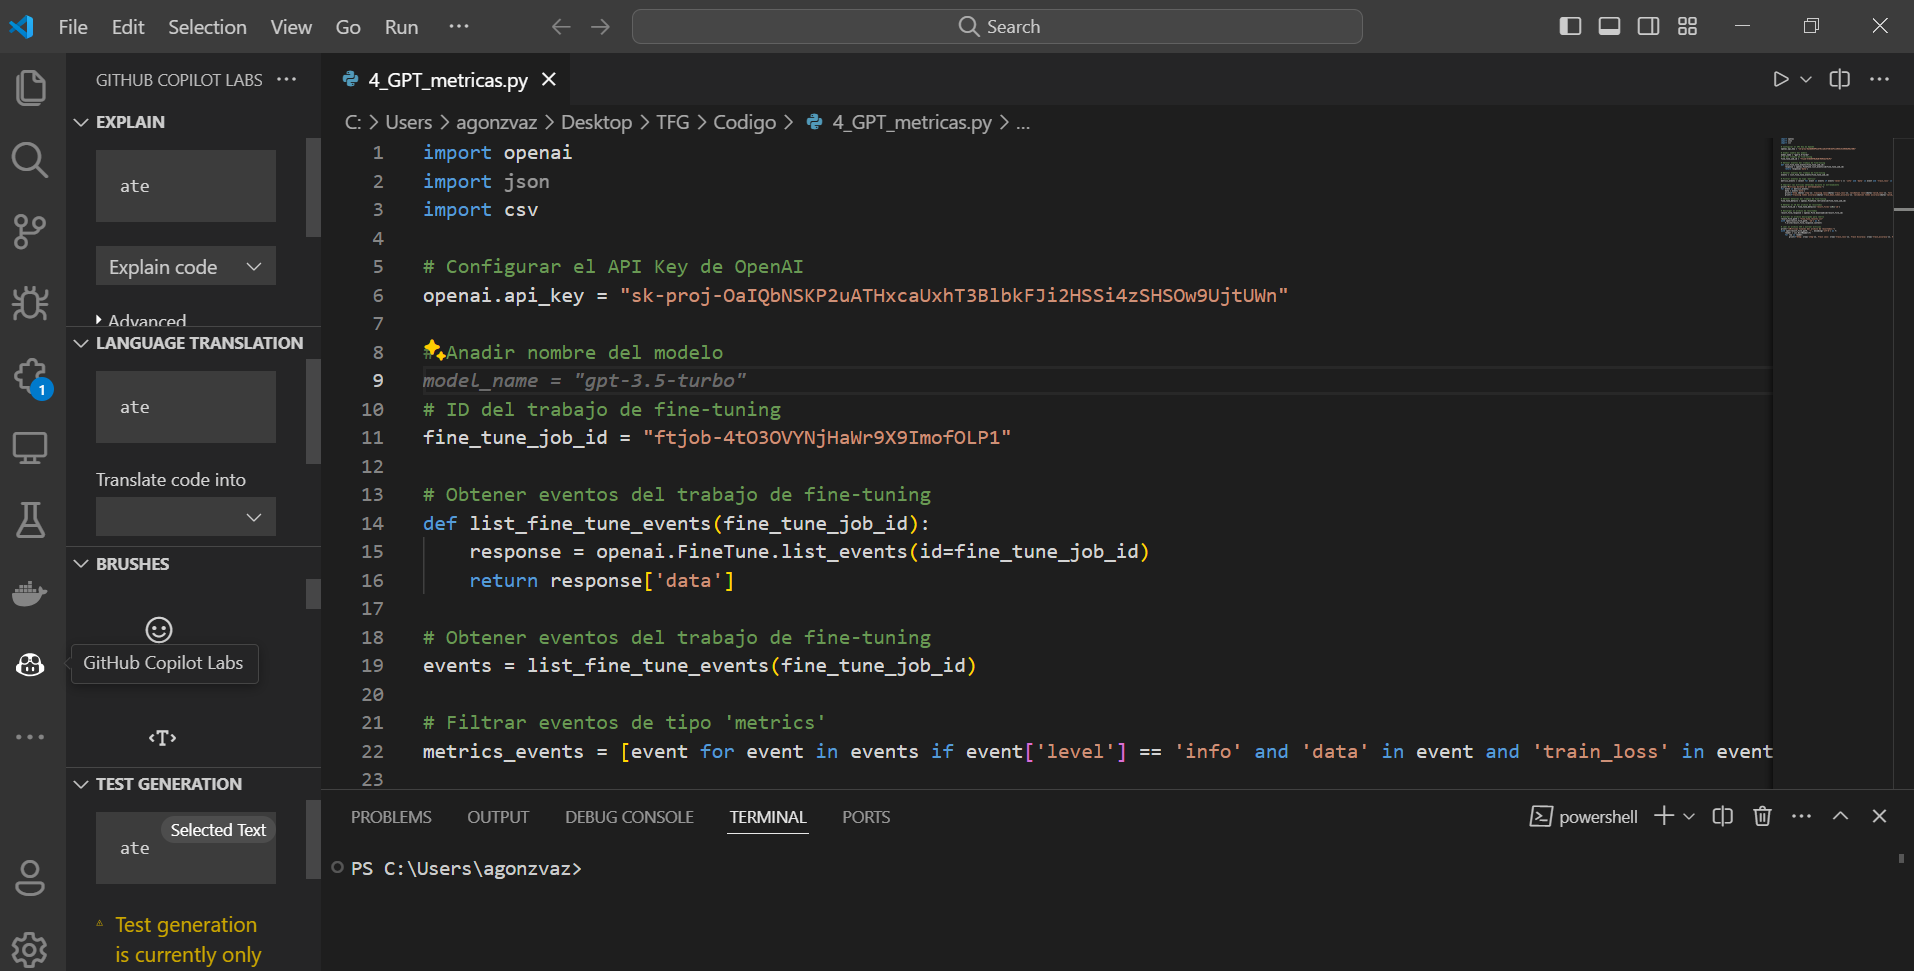
\includegraphics[width=1\textwidth]{imaxes/1_MuestraCopilot.png}
\caption{Ejemplo práctico del funcionamiento de GitHub Copilot.}
  \label{fig:1_MuestraCopilot}
\end{figure}


\section{OpenAI Codex}

OpenAI Codex \cite{OpenAICodex}, desarrollado por OpenAI, es una herramienta que interpreta el lenguaje natural y genera código. Codex, basado en el exitoso GitHub Copilot, es un producto generado a partir del modelo \acrshort{GPT}-3 de OpenAI, creado específicamente para emplearse en tareas de programación. Su lanzamiento en una fase beta exclusiva ha sido respaldado por una extensa capacitación en 159 GB de código Python extraído de 54 millones de repositorios en GitHub.

Codex hace más fácil escribir código al ofrecer sugerencias específicas y adecuadas, y también puede comprender y seguir instrucciones en lenguaje natural. Gracias a su capacidad para aprender varios lenguajes de programación, es capaz de participar en diferentes proyectos de desarrollo de software. La \acrshort{API} exclusiva de Codex permite cambiar la forma en que los desarrolladores interactúan con el software al integrar funciones de generación de código, acelerando la creación y fomentando la innovación en programación.